\section{Interfejs użytkownika}
Interfejs użytkownika aplikacji składa się z kilku głównych widoków, które umożliwiają użytkownikom korzystanie z różnych funkcji. Wszystkie widoki zostały zaprojektowane z myślą o prostocie i intuicyjności, aby zapewnić użytkownikom łatwą nawigację i szybki dostęp do potrzebnych informacji. Poniżej przedstawiono najważniejsze elementy interfejsu użytkownika.


\subsection{Widok startowy}

\begin{figure}[H]
    \centering
    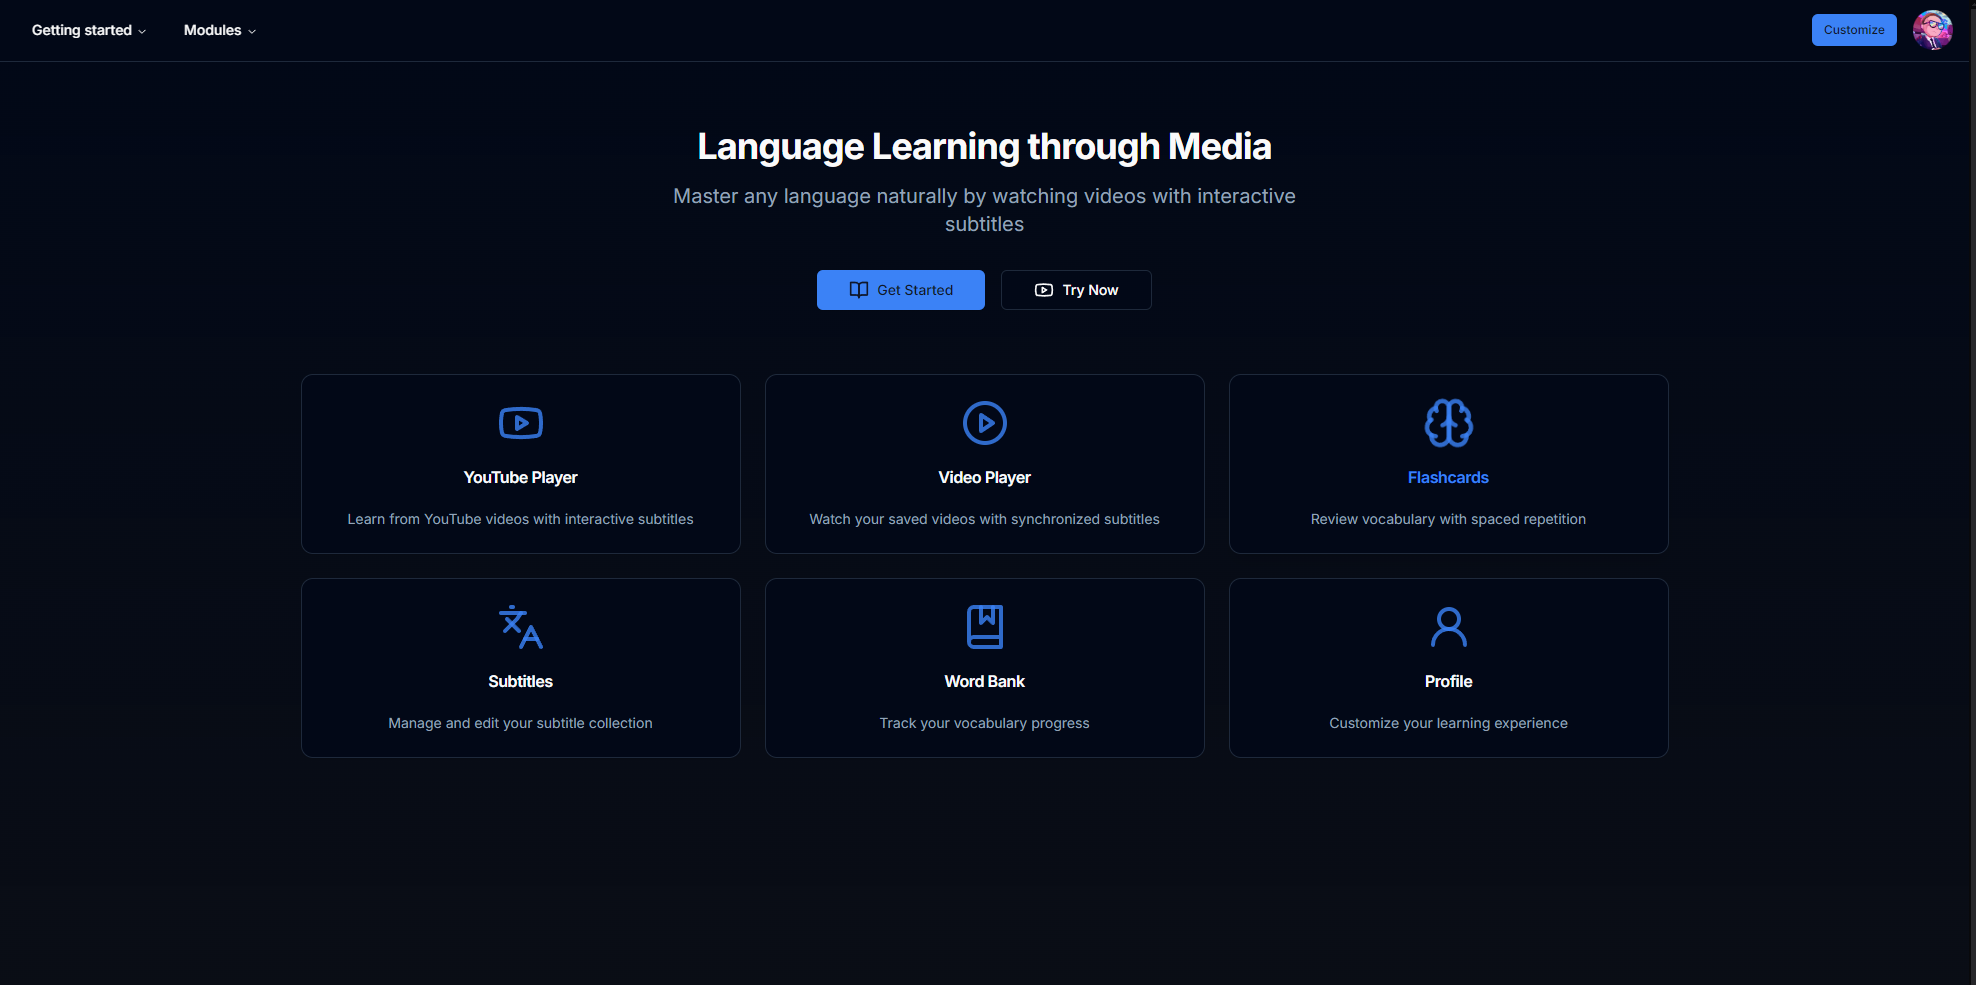
\includegraphics[width=1\textwidth]{IMAGE/HomePage.png}
    \caption{Strona główna aplikacji}
    \label{fig:Widok strony głównej aplikacji}
\end{figure}
Strona główna aplikacji zawiera przyciski kierujace do innych sekcji aplikacji, takich jak nauka, słownik, statystyki, profil użytkownika, ustawienia, itp. Użytkownicy mogą również przeglądać najnowsze filmy i seriale dostępne w aplikacji oraz korzystać z wyszukiwarki, aby znaleźć interesujące ich treści.

\subsection{Strona Nauki}

\begin{figure}[H]
    \centering
    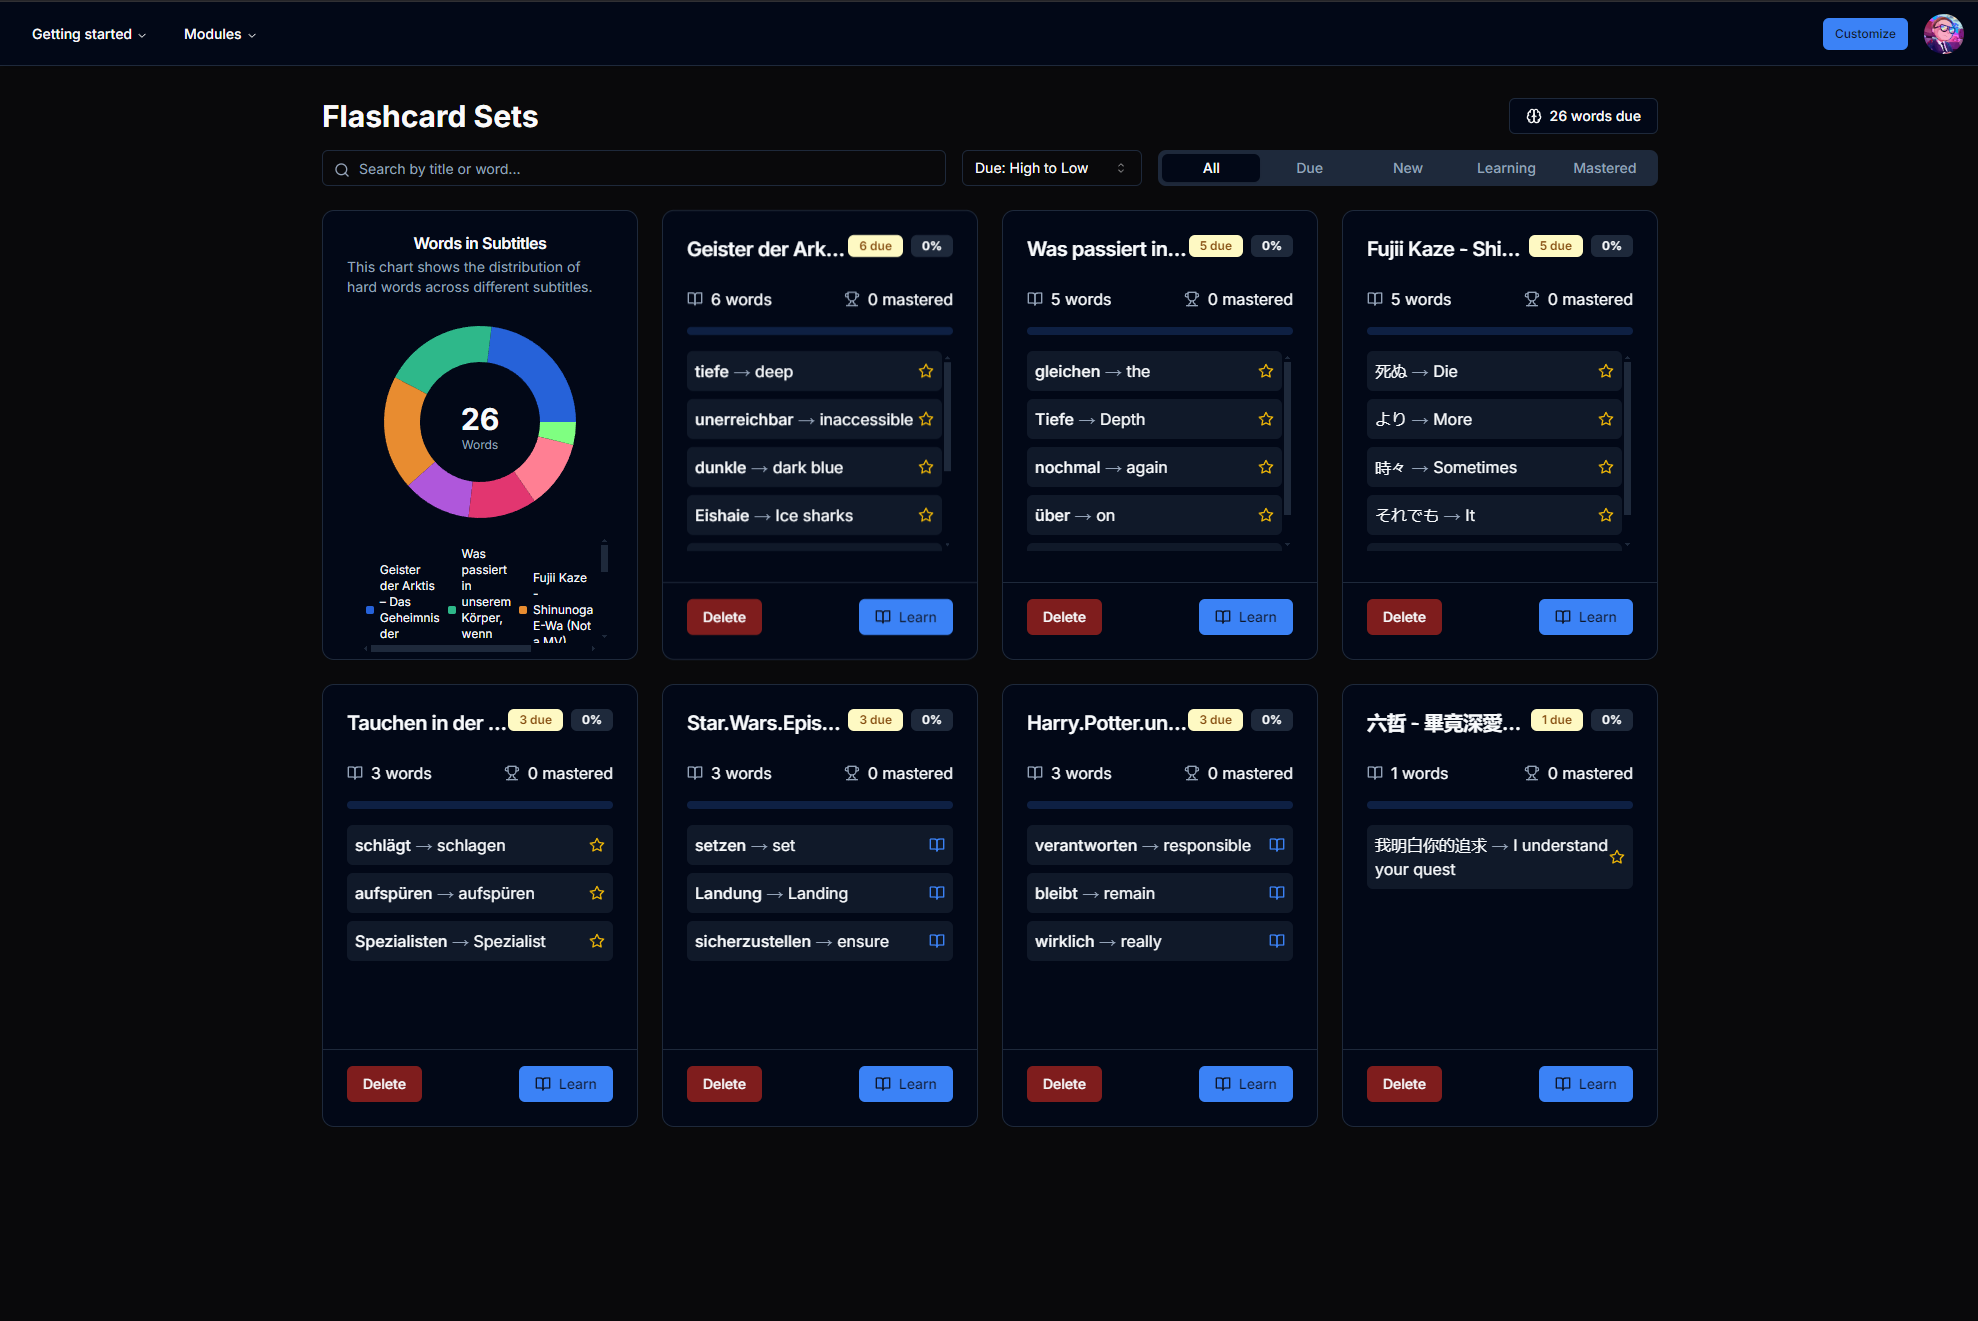
\includegraphics[width=1\textwidth]{IMAGE/FlashCards.png}
    \caption{Widok strony głównej fiszek}
    \label{fig:Strona głowna fiszek}
\end{figure}
\begin{figure}[H]
    \centering
    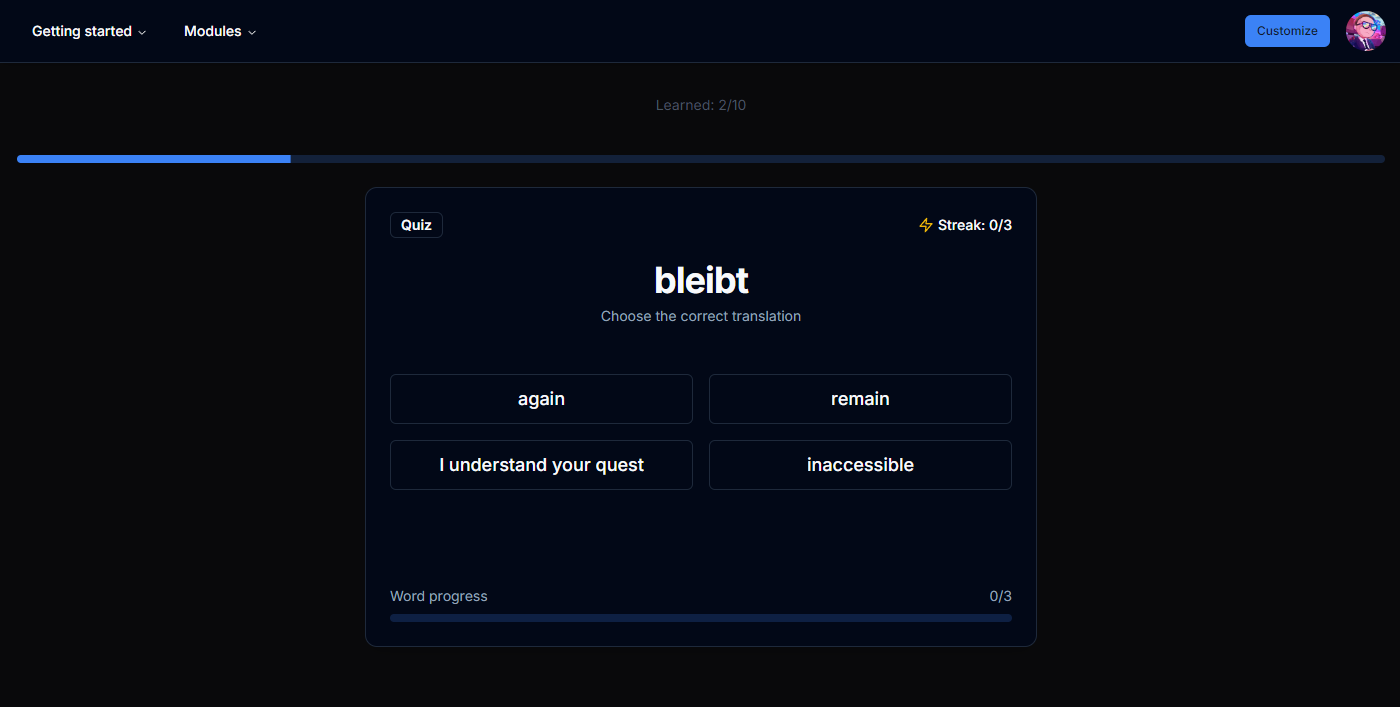
\includegraphics[width=1\textwidth]{IMAGE/Quiz.png}
    \caption{Widok quizu}
    \label{fig:Nauka z quizem}
\end{figure}
Strona Nauki to główne miejsce, w którym użytkownicy mogą korzystać z panelu nauki fiszek lub quizu. Panel fiszek zawiera informacje na temat stanu słów które są nowe, w trakcie nauki, lub skończone. Strona quizu umożliwia użytkownikom nauke poprzez quizy, w których użytkownicy muszą wybrać poprawne tłumaczenie słowa. Użytkownicy muszą poprawnie odpowiedzieć 3 razy z rzędu by słowo zostało uznane za nauczone i przeszło do kolejnego etapu którym jest powtórka po upływie odpowiedniego czasu \cite{mallett2012benefits}.

\subsection{Strona Napisów}

\begin{figure}[H]
    \centering
    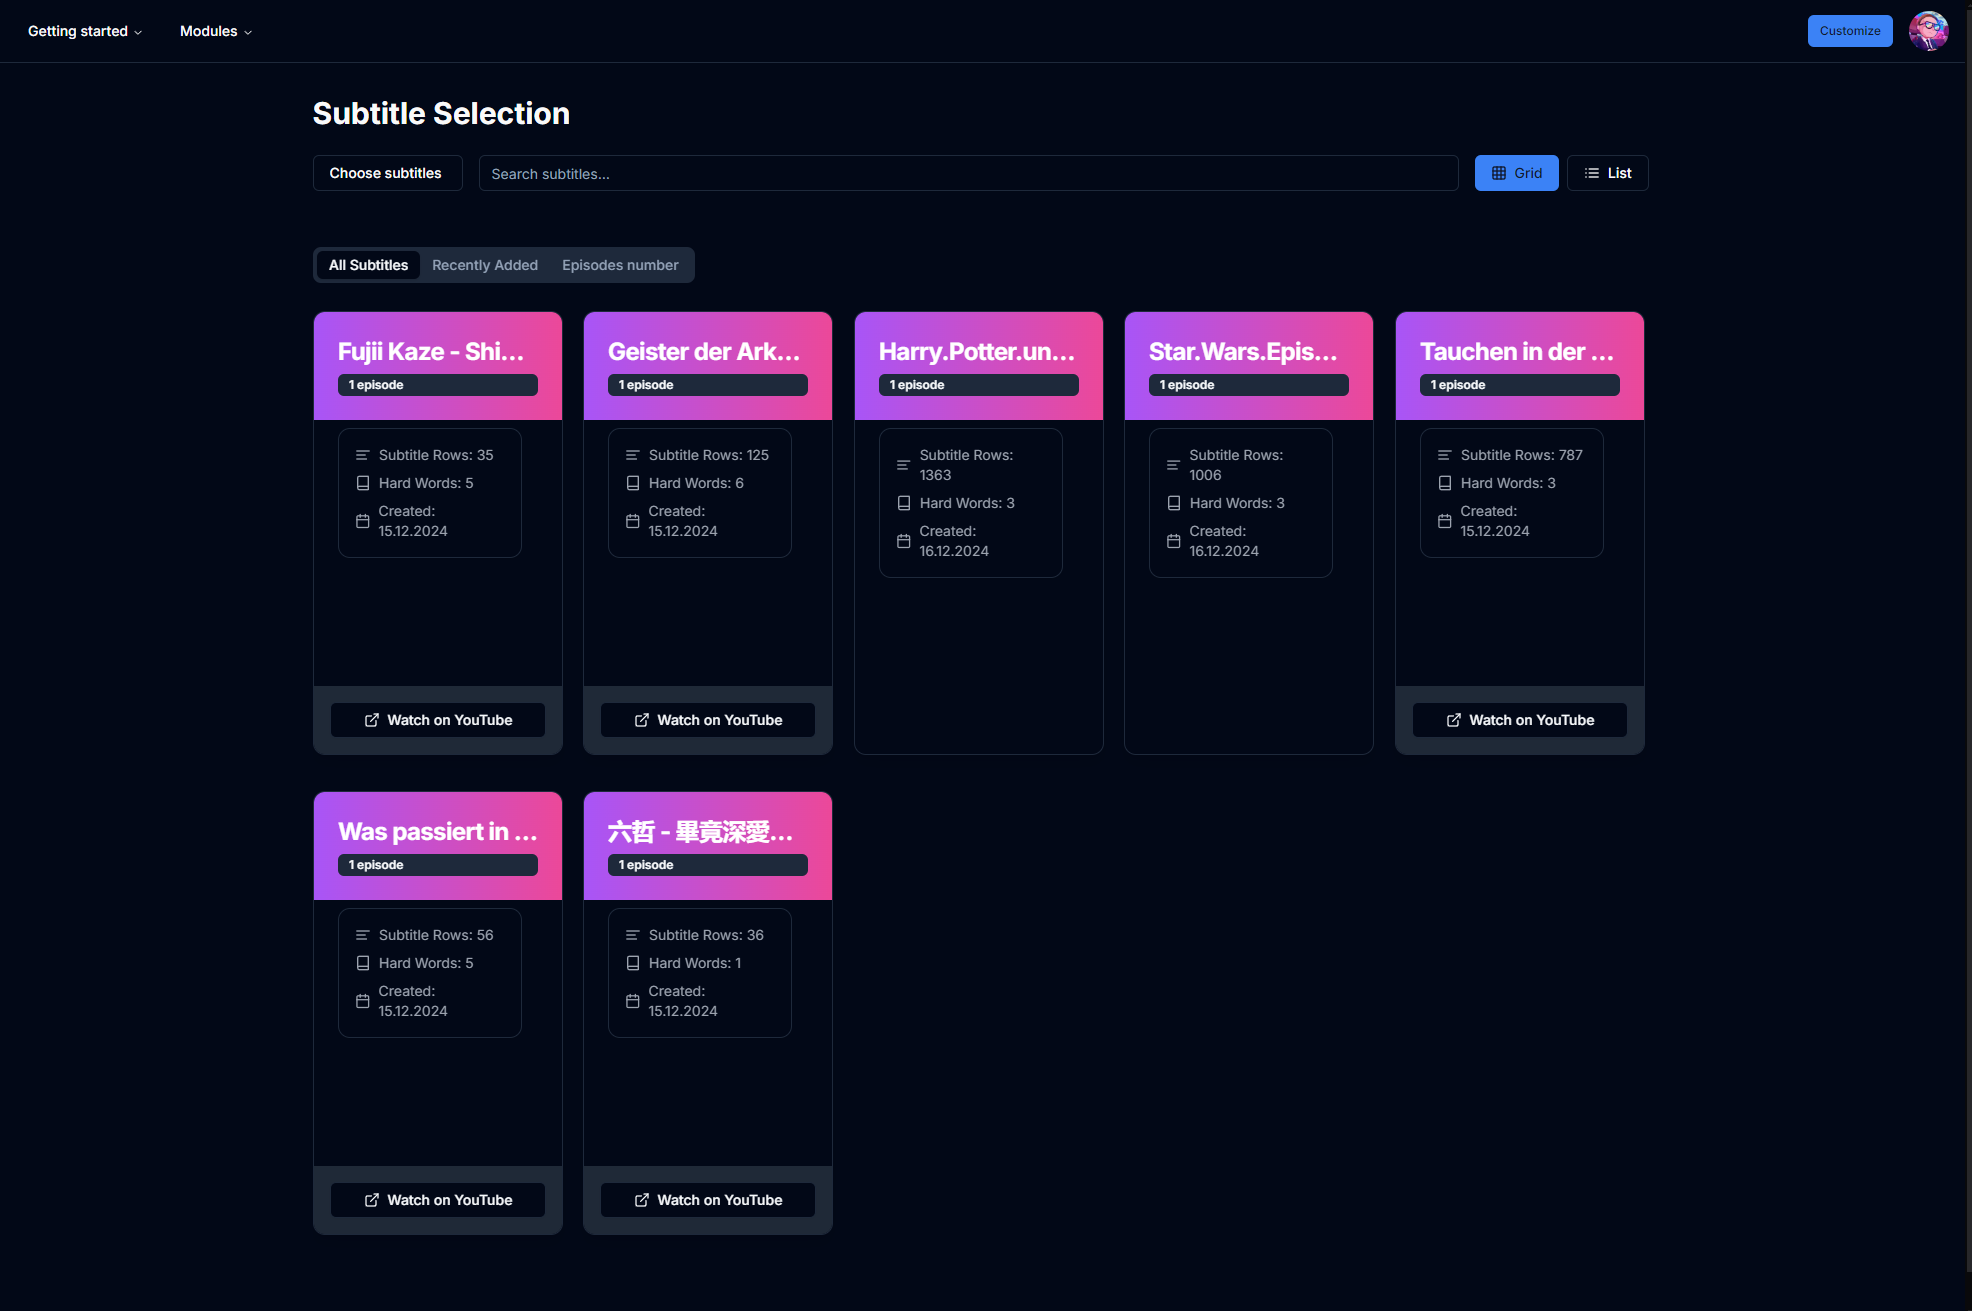
\includegraphics[width=1\textwidth]{IMAGE/Subtitles.png}
    \caption{Widok strony napisów}
    \label{fig:Strona napisów}
\end{figure}
Strona główna umożliwia wyszukiwanie zapisanych napisów, dostępne jest wyszukiwanie po tytule. Użytkownicy mogą również sortować napisy według daty dodania oraz liczby odcinków. Panel daje również możliwość zmiany wyświetlania między siatką a listą domyślnie jest to siatka maksymalnie 5 elementów na wiersz w zależności od miejsca na ekranie.

\begin{figure}[H]
    \centering
    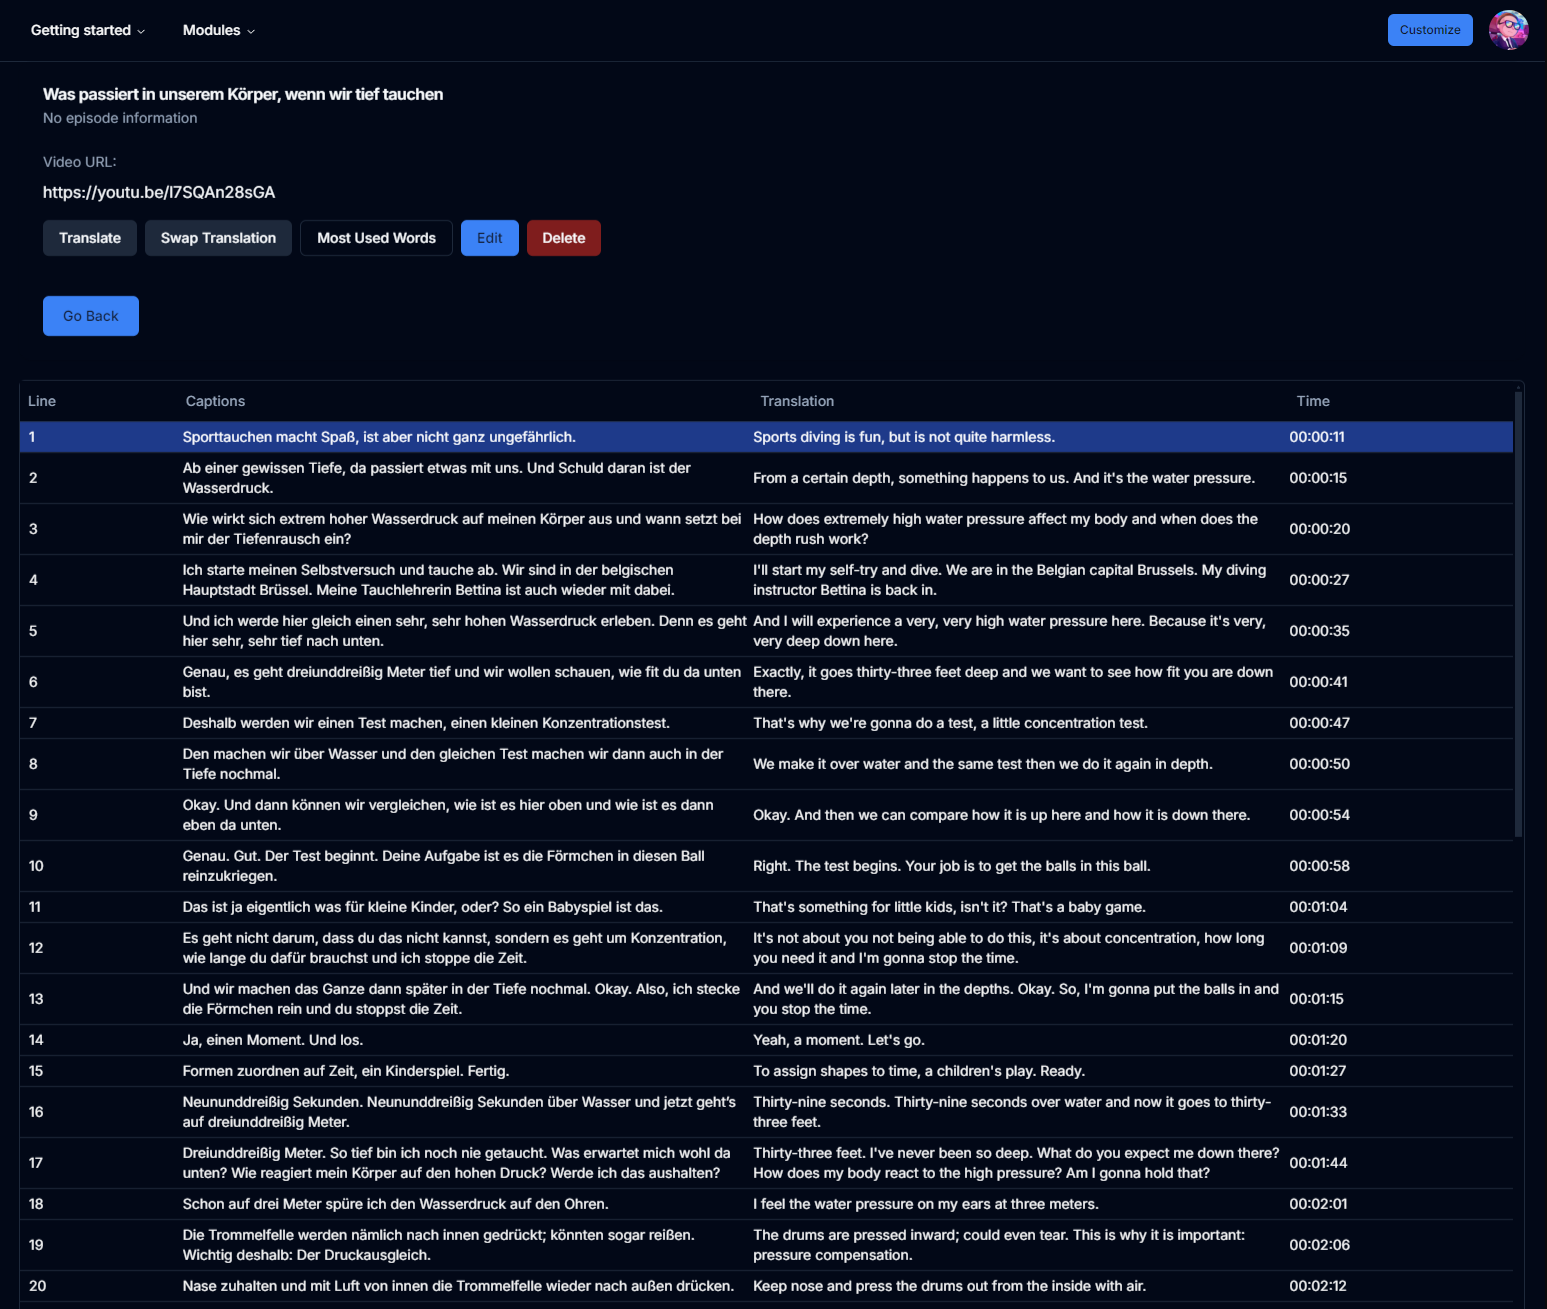
\includegraphics[width=1\textwidth]{IMAGE/SubtitlesSelected.png}
    \caption{Widok edycji napisów}
    \label{fig:Edycja napisów}
\end{figure}
Strona Napisów umożliwia użytkownikom przeglądanie i edycję napisów w bazie danych. Użytkownicy mogą edytować istniejące napisy, usuwać napisy, a także przeglądać listę wszystkich napisów w bazie z pomocą sortowania i wyszukiwania.

\subsection{Strona Słownika}

\begin{figure}[H]
    \centering
    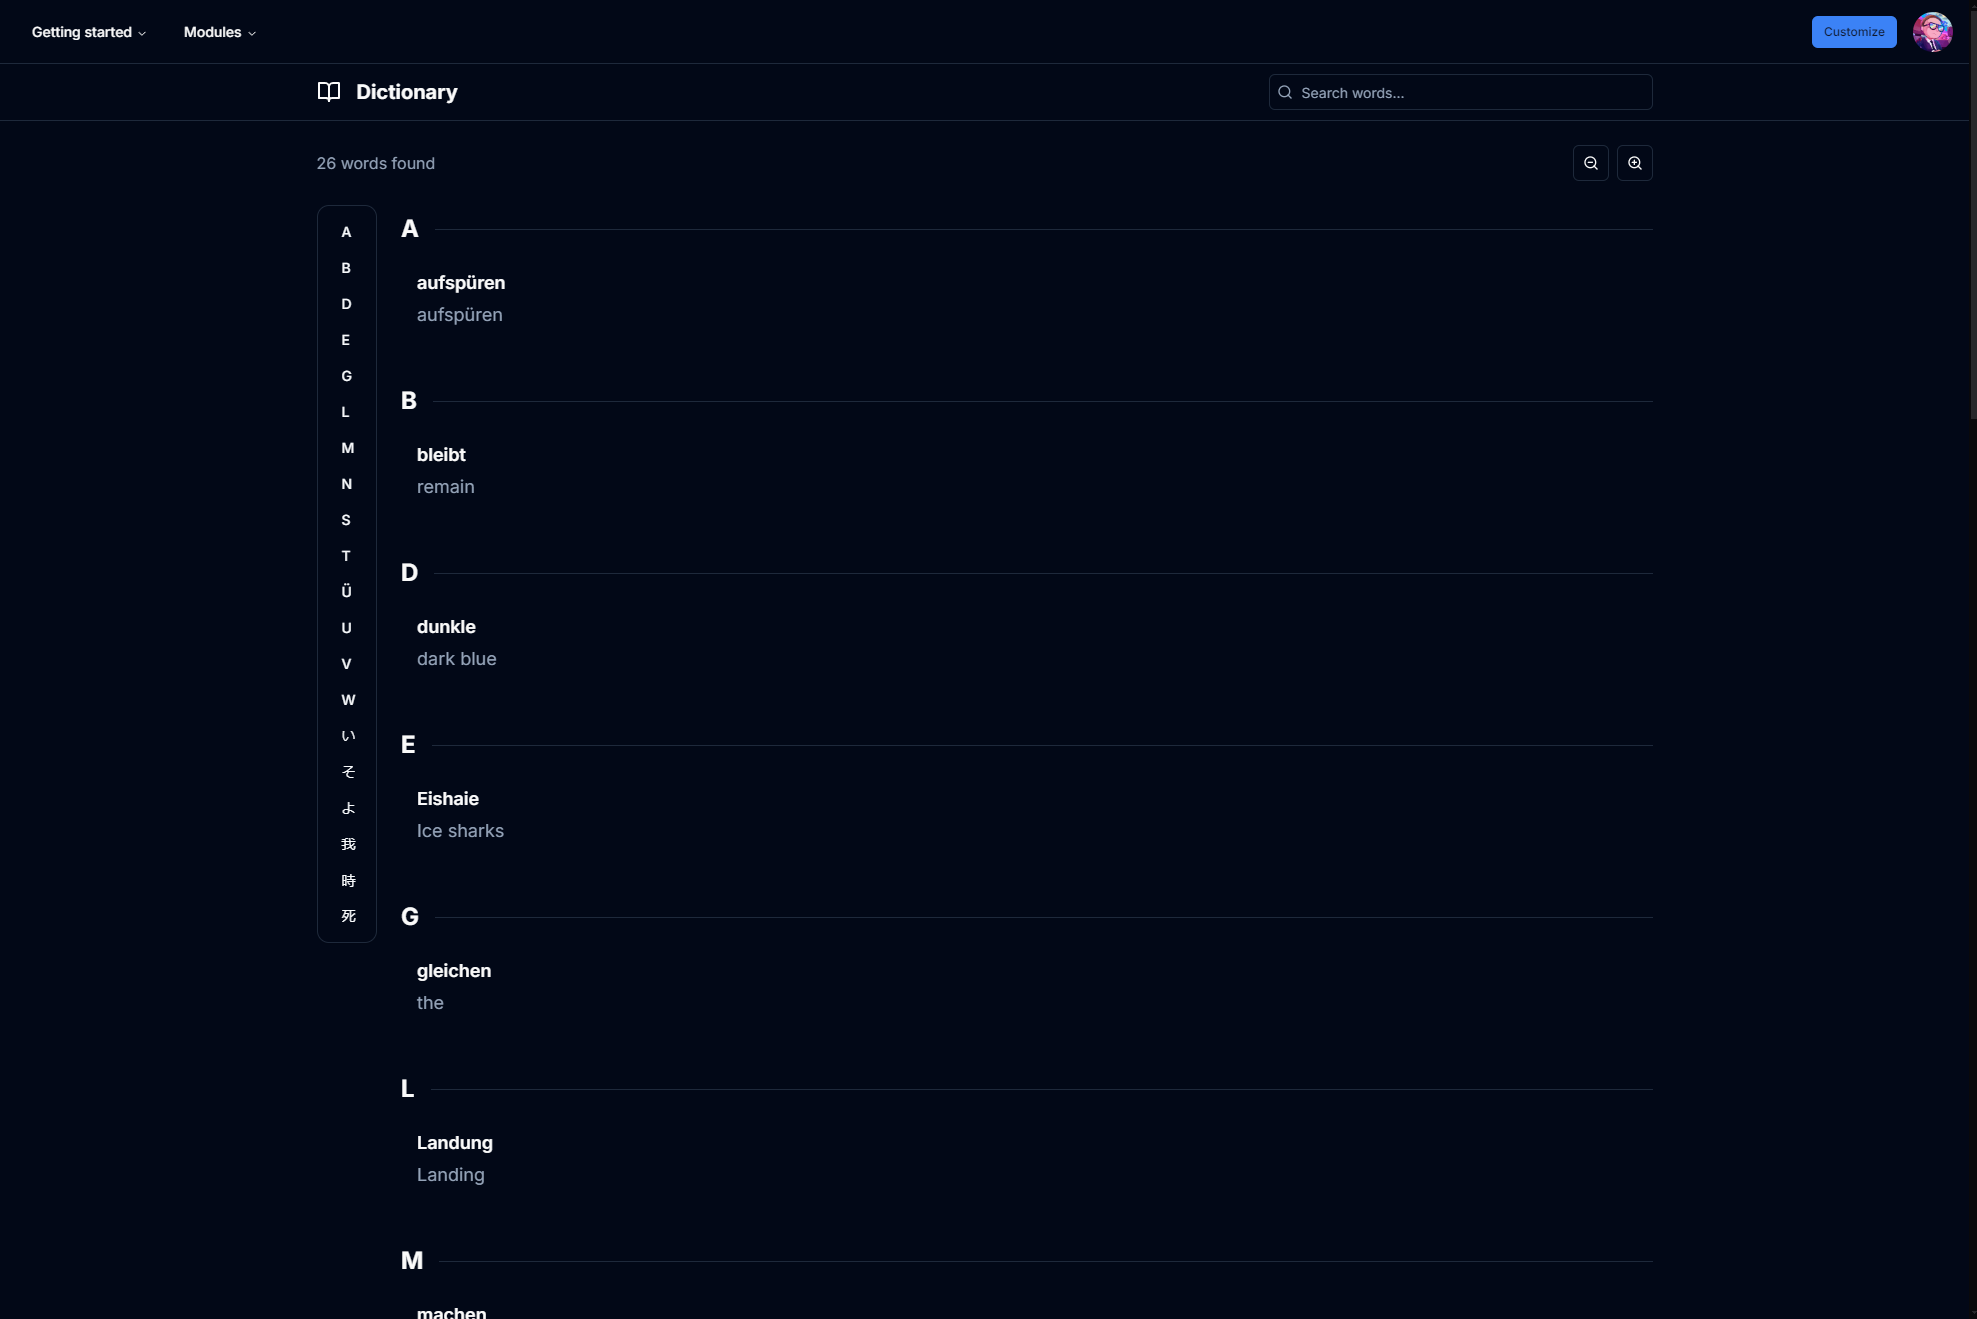
\includegraphics[width=1\textwidth]{IMAGE/WordBank.png}
    \caption{Widok słownika}
    \label{fig:Słownik słów}
\end{figure}
Strona Słownika umożliwia użytkownikom przeglądanie i edycję słów w bazie danych. Użytkownicy mogą  edytować istniejące słowa, usuwać słowa, a także przeglądać listę wszystkich słów w bazie z pomocą sortowania i wyszukiwania. Panel obsługuje również chińskie znaki.
\subsection{Strona Statystyk}

\begin{figure}[H]
    \centering
    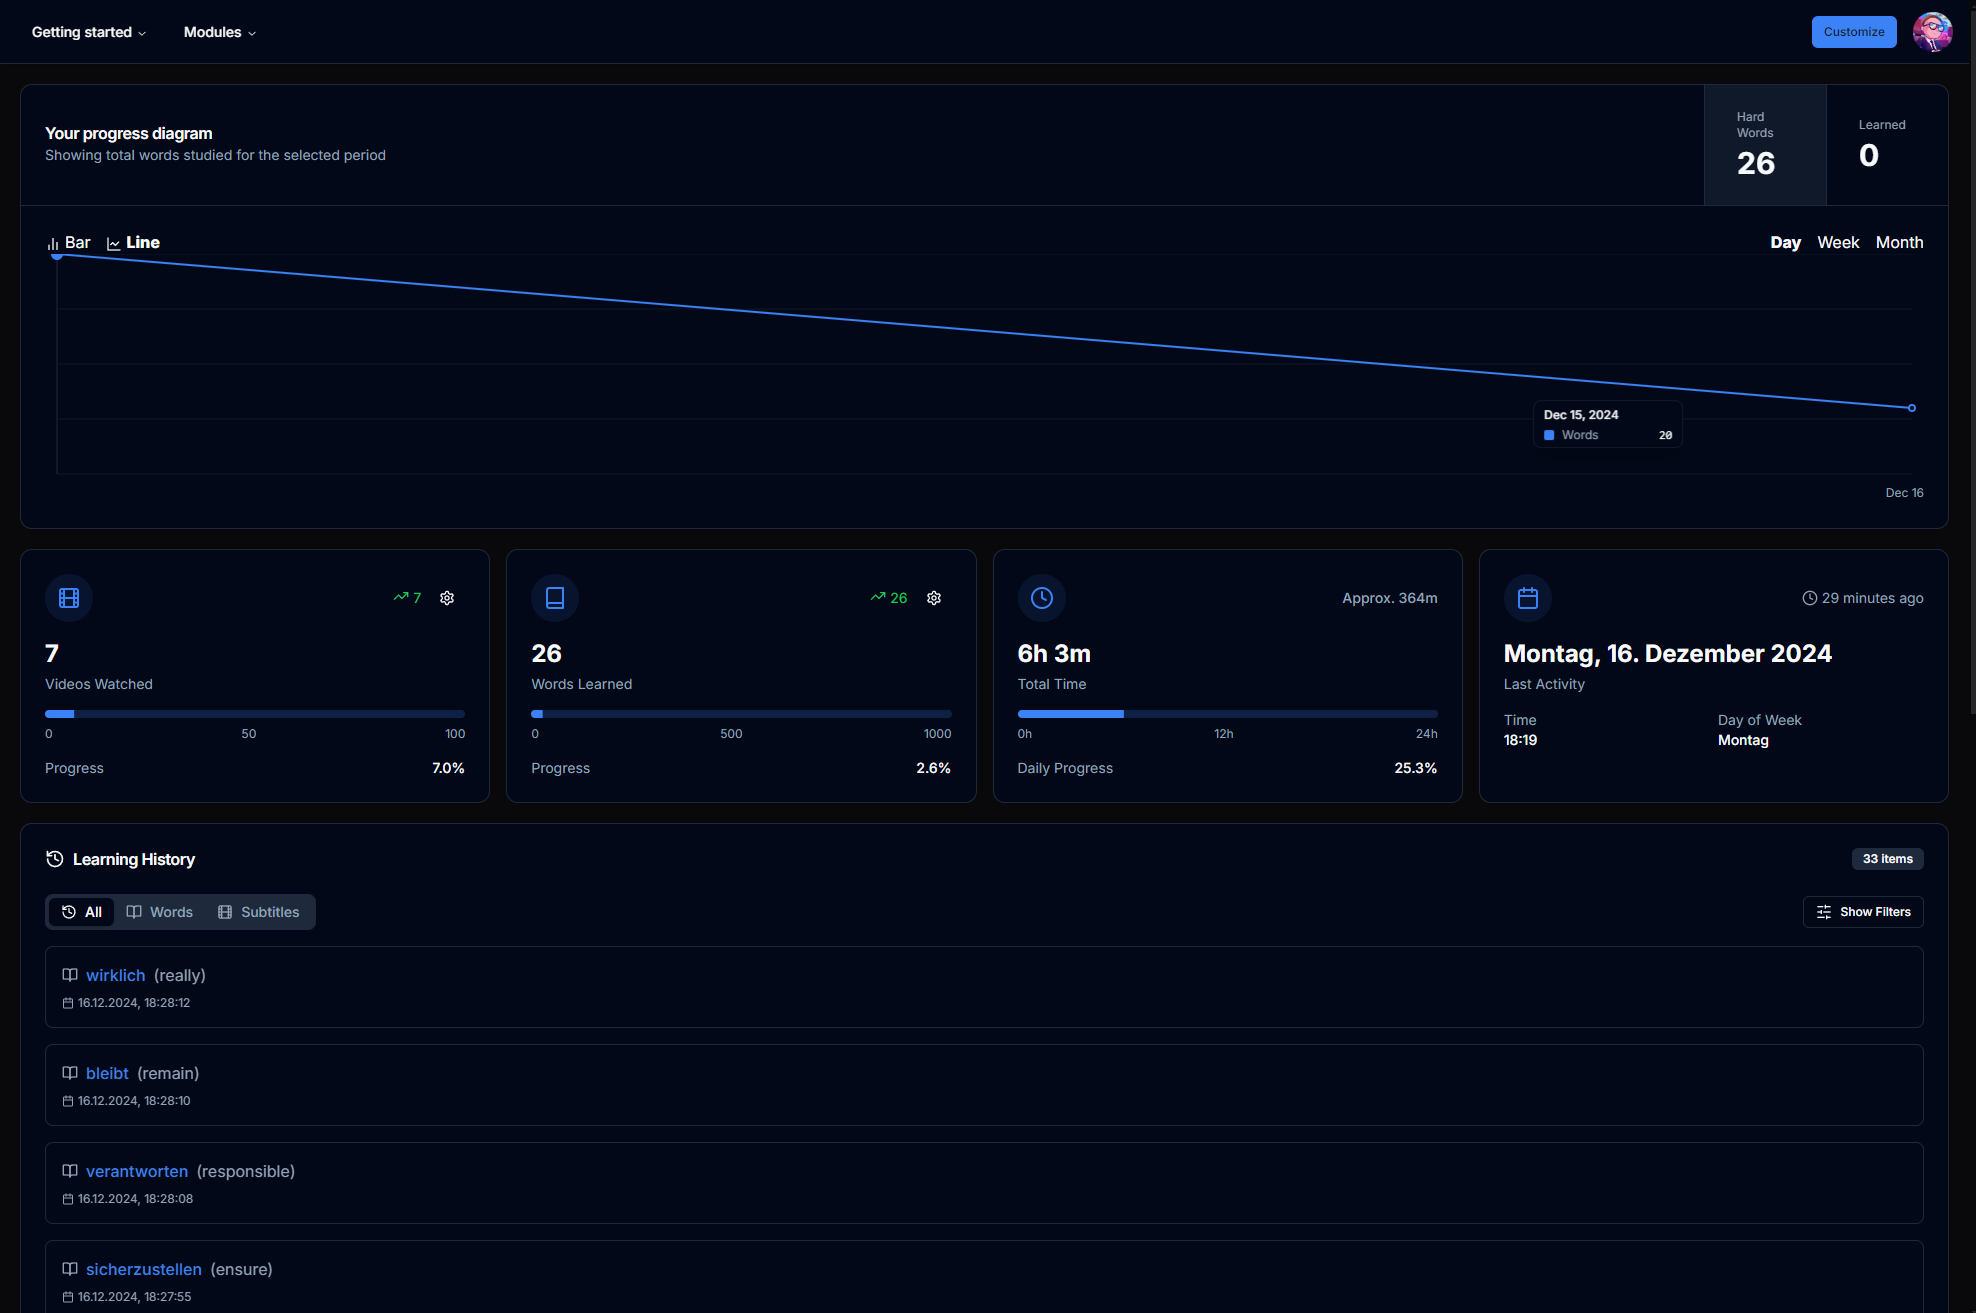
\includegraphics[width=1\textwidth]{IMAGE/Progress.png}
    \caption{Widok statystyk i postępów}
    \label{fig:Statystyki postępów}
\end{figure}
Strona Statystyk zawiera wykresy i statystyki dotyczące postępów w nauce użytkowników. Użytkownicy mogą śledzić swoje postępy w nauce słówek. Panel zawiera również informacje na temat liczby nowych słówek, oraz słówek nauczonych już wraz z datami utworzenia słowa i ukończenia nauki.
\subsection{Strona logowania oraz rejestracji}

\begin{figure}[H]
    \centering
    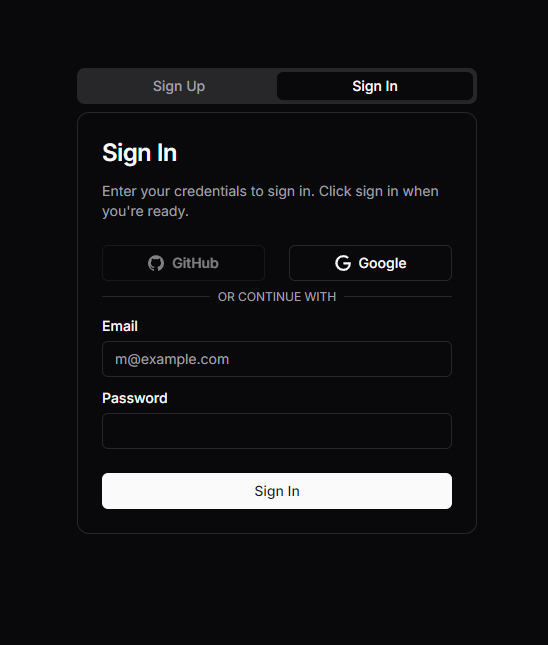
\includegraphics[width=1\textwidth]{IMAGE/LoginPage.png}
    \caption{Widok logowania i rejestracji}
    \label{fig:Logowanie i rejestracja}
\end{figure}
Strona logowania i rejestracji umożliwia użytkownikom zalogowanie się do aplikacji lub utworzenie nowego konta. Użytkownicy mogą wprowadzić swoje dane logowania, takie jak adres e-mail i hasło, aby uzyskać dostęp do aplikacji. Panel obsługuje również logowanie za pomocą konta Google, Logowanie za pomocą GitHub będzie dodane również pózniej.
\subsection{Strona oglądania filmów}


\begin{figure}[H]
    \centering
    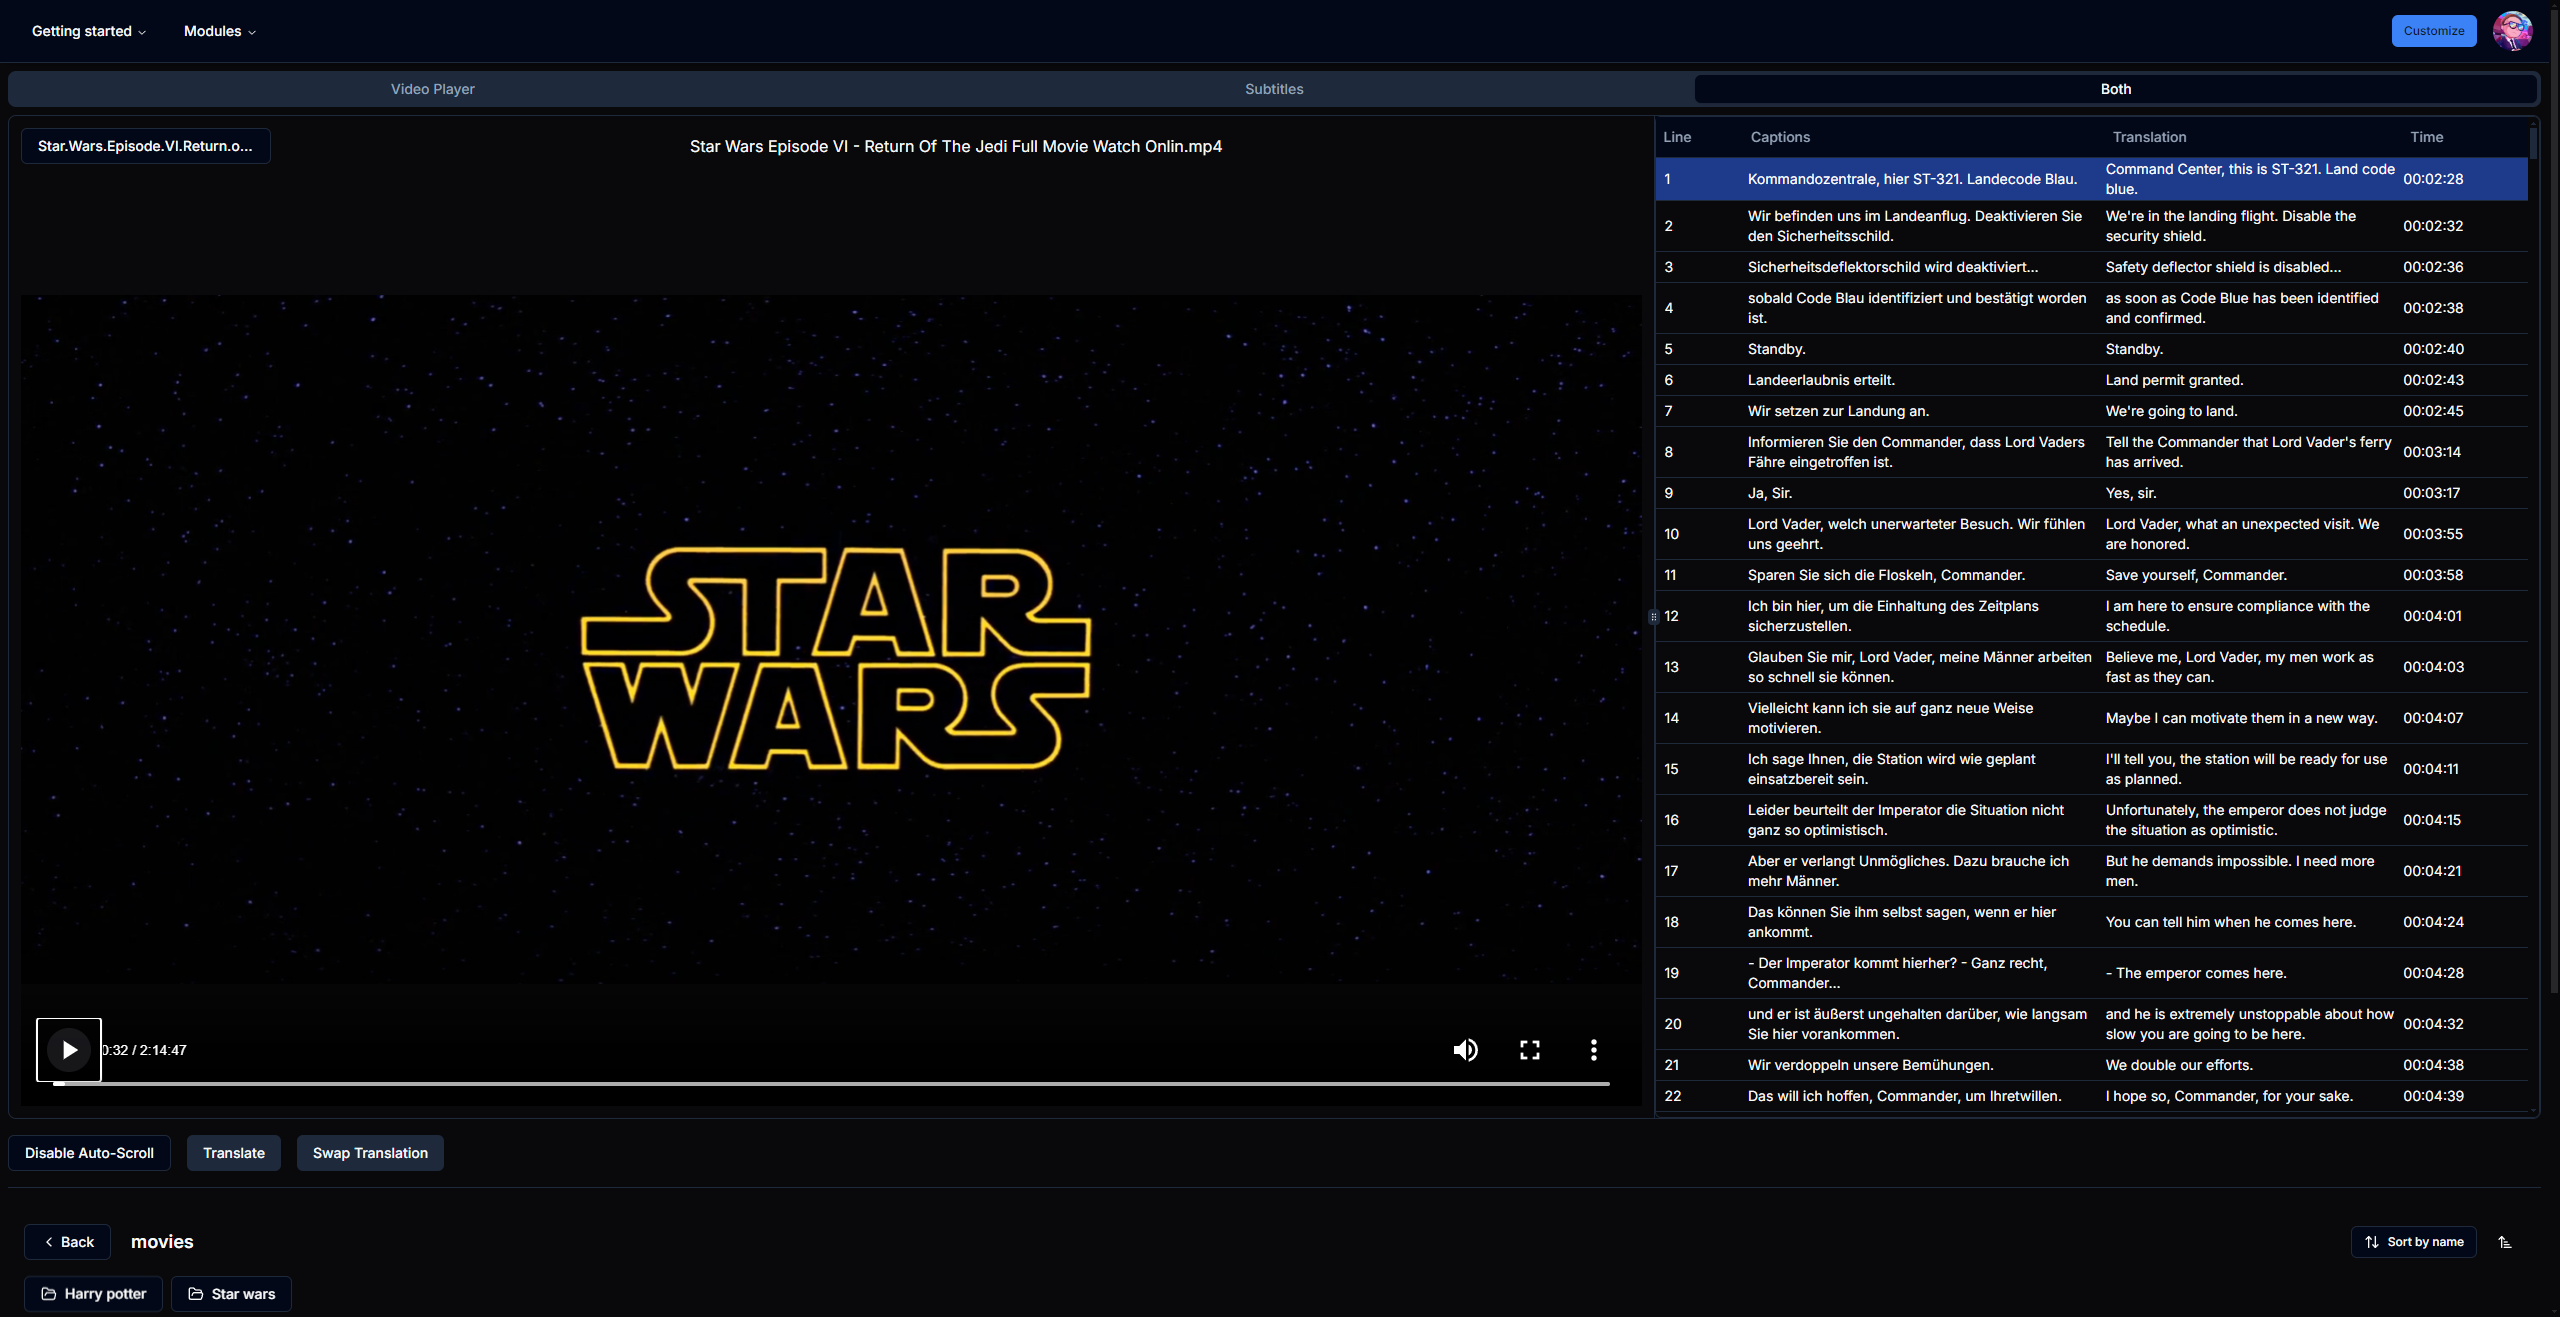
\includegraphics[width=1\textwidth]{IMAGE/videoPlayer.png}
    \caption{Widok oglądania filmów}
    \label{fig:oglądanie filmów}
\end{figure}

Strona oglądania filmów umożliwia użytkownikom przeglądanie i odtwarzanie filmów i seriali z listy zapisanych napisów i wybrania odpowiedniego filmu z dysku. Użytkownicy mogą zamienić szybko jezyk orginalny z przetłumaczonym lub włączyć śledzenie aktualnego wiersza napisów względem filmu "auto-scroll", a następnie rozpocząć oglądanie. Panel obsługuje również przewijanie filmu, zmianę języka napisów, oraz dodawanie słów do bazy w celu pózniejszej nauki. Użytkownik ma do wyboru albo filmy z rozszerzeniem mp4 albo mkv a napisy w formacie srt lub ass.

